%&<tex>
\documentclass[12pt,a4paper, onecolumn]{IEEEtran}
%\documentclass[conference]{ieeeconf}
%\IEEEoverridecommandlockouts    % This command is only needed if you need \thanks
\usepackage{./bibNmacro/sauravMacros}
%\documentclass[number,sort&compress, 1p]{elsarticle}
%\usepackage{epsfig}
%\usepackage{helvet}
%\usepackage{courier}
%\usepackage{amsmath,amsfonts}
%\usepackage[bottom]{footmisc}
%\usepackage{amssymb}
\usepackage{booktabs}
\usepackage{graphics,graphicx}
%\usepackage{subfigure}
%\usepackage{subcaption}
%\usepackage{xspace}
%\usepackage{qtree} % check if needed 
%\usepackage{url}  
\usepackage{color, soul}
%\usepackage{gensymb}
\newcommand{\fgref}[1]{Fig.~\ref{#1}}
%\usepackage{xparse}
%\usepackage{threeparttable}
\usepackage{fancyhdr}
\usepackage{lastpage}
\usepackage{float}
\usepackage[]{algorithm2e}
%\newtheorem{lemma}{Lemma}
%\newtheorem{remark}{Remark}
%\usepackage{amsthm}
%\usepackage{siunitx}
%\renewcommand{\headrulewidth}{0pt}
%\pagestyle{fancy}
%\fancyhf{}
%\usepackage{widetext}
%\usepackage{multirow}
%\usepackage{enumerate}
%\newcommand{\bs}[1]{{\boldsymbol{#1}}}
\usepackage{hyperref}
\usepackage{xcolor}
\newcommand{\hlc}[1]{{%
    \colorlet{foo}{cyan!50}%
    \sethlcolor{foo}\hl{#1}}%
}
\hypersetup{
  colorlinks,
  linkcolor={red!50!black},
  citecolor={red!60!black},
  urlcolor={blue!80!black}
}
\usepackage{authblk}
% Following macros have been moved to sauravMacros.sty
%\newcommand{\sac}[1]{{\color{blue!80!black} [Saurav: {\em #1}]}\xspace}
%\newcommand{\sak}[1]{{\color{red!80!black} [Srinivas: {\em #1}]}\xspace}
%\newcommand{\mv}[1]{\mathbf{#1}}
%%%%%%%%%%%%%%%%%%%%%%%%%%%

\newcommand{\vpi}{\mv p_i}
\newcommand{\vsj}{\mv s_j}
\newcommand{\vqj}{\mv q_j}
\newcommand{\vdo}{\mv d_0}
%\newcommand{\vn}[1]{#1^{\top}#1}
%\newcommand{\vnt}[2]{#1^{\top}#2}
%\newcommand{\sumn}[1]{\sum_{#1=1}^{n}}
%\renewcommand{\eqref}[1]{Eq.~(\ref{#1})}

\pdfminorversion=4

%\newtheorem{lem}{Lemma}
%\headheight 15pt
%\textheight 10in %7.75in
%\topmargin -1in
%\textwidth 6.5in
%\oddsidemargin 0in
%\evensidemargin 0in
%\footskip 0.5in
% \parindent 0.25in
% \lineskip 1pt
% \normallineskip 1pt
% \def\baseltioinestretch{1.5}
%\newcommand{\meqref}[1]{Eqs.(#1)}
\usepackage[normalem]{ulem}  % for \sout{}
\graphicspath{{./graphics/}}
\author{Saurav Agarwal
  \thanks{Department of Computer Science, University of North
  Carolina at Charlotte, NC 28223, USA.}%
  \thanks{{\tt \small sagarw10@uncc.edu, 800965622}} % Corresponding author

}
\begin{document}
%\rmdefault
\title{{\Large \bf Path Planning for Multiple Robots with Variable Formation Using
Probabilistic Roadmap}\\{\large ITCS-8152: Robot Motion Planning} {\large (Spring 2018)} }
%\title{Simultaneous Optimal Assignment and Goal Formation for Multiple Robots}
%\title{Assignment and Trajectory Planning for Multiple Robots with Variable Goal Formations}
\maketitle
%\rhead{Page \thepage \hspace{1pt} of \pageref{LastPage}}
%%%%%%%%%%%%%%%%%%%%%%%%%%%%%%%%%%%%%%%%%%%%%%%%%%
\begin{abstract}
%
  The objective of the project is to implement and analyze Probabilistic Road Map (PRM) algorithm for motion planning of multiple robots with variable formation. By variable formation we mean that the robots can change the scale and orientation of the formation while maintaining a given shape. The system of robots hence have five degrees of freedom, i.e., three for translation, scale, and orientation about the $Z$-axis. The PRM algorithm is implemented as it can handle high dimensional configuration space. Additional connectivity, expansion, and smoothing techniques are implemented to improve upon the solutions generated. Examples of different numbers of robots in various shapes are considered to analyze the efficacy of the algorithm. The algorithm is implemented using Python 2.7 and Klamp't motion planning framework.
\end{abstract}
%%real-time applications. 
%% and implementations on a team of Turtlebot2 robots 

%%%%%%%%%%%%%%%%%%%%%%%%%%%%%%%%%%%%%%%%%%%%%%%%%
\section{Introduction}
%\section{Motivation}
%
Teams of robots often maintain a desired shape while performing tasks such as exploration,
coverage, and surveillance~\cite{TurpinMK12ICRA}. These formations can have the
flexibility in the scale and orientation of the formation while maintaining the given
shape. These additional degrees of freedom allows us to navigate through narrow passages
in the environment (see~\fgref{fig:r200}). In this project we study an analyze the
Probabilistic Roadmap path planning method to perform path planning in
a static environment with obstacles.

\begin{figure}[htbp]
  \centering
  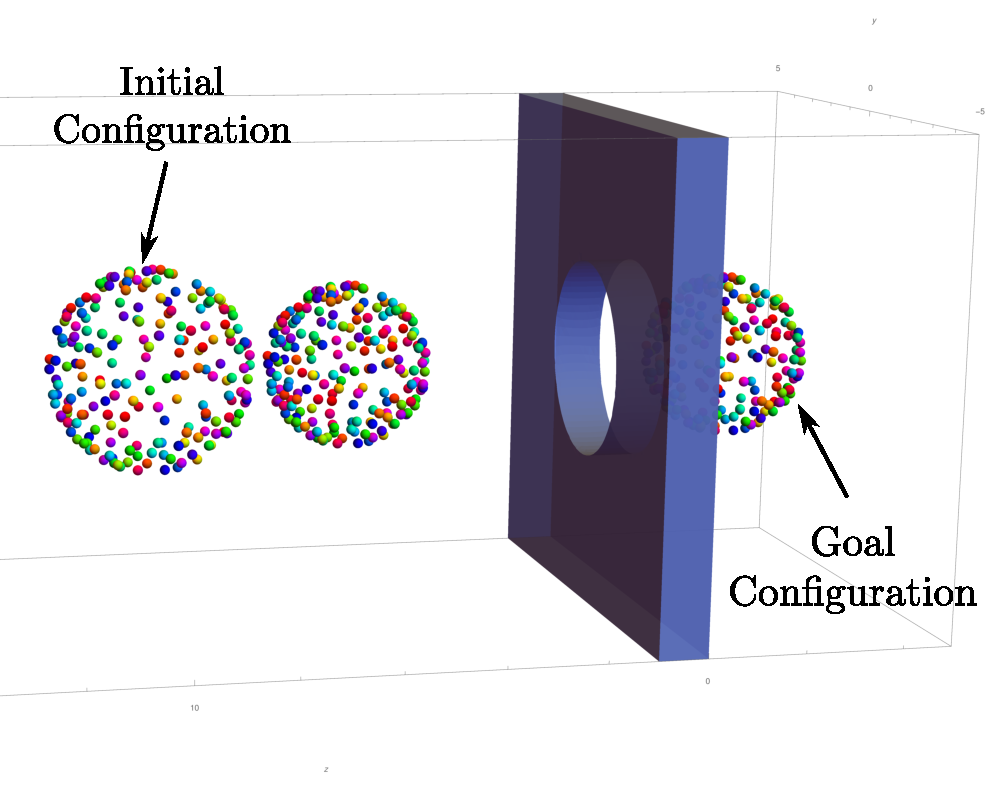
\includegraphics[width=0.5\textwidth]{r200_all}
  \caption{An example of a scenario where robots need to change their scale in order to
  pass through a narrow opening. We need to ensure that the scale parameter is computed
  such that the robots do not collide with
themselves.}
  \label{fig:r200}
\end{figure}


Several efficient path planning techniques exist for low dimensional configuration space. Roadmap methods in $\mathbb R^2$ include visibility graph, which can give optimal paths, Voronoi
roadmap which keep the path far away from the obstacles (along the medial axis). Cell
decomposition methods divide the free configuration space of the robots into cells.
Thereafter, a connectivity graph is created to with the cells. Given query points, a path
is found in the connectivity graph. These methods can solve 2D configuration spaces
efficiently. However, the as the dimension increases, the number of cells increases
exponentially and both the space and time complexity increases. Potential field methods is
another class of motion planning technique wherein potential functions dictate the
motion of the robots. The goal position has an attractive potential and the obstacles
(potentially other robots as well) have repulsive potential. The forces on the robot are
then computed based on the potential function. The method suffers from getting stuck at
local minima and designing potential navigation functions may not be trivial. 

All the algorithms discussed above do not perform well when the dimension of the
configuration space increases. In general the motion planning problem is PSPACE-hard.
Owing to this difficult, in the past decade there have been significant advances in
sampling based techniques. One such method is Probabilistic Roadmap
(PRM)~\cite{kavrakiSLO96} composed of a
learning phase and a query phase. The learning phase builds a roadmap and in the query
phase shortest path in computed in the roadmap. The PRM has been shown to be effective in
various environments with high dimensional configurations of robots. There have been
several improvements and variants to PRM. One notable improvement is
PRM*~\cite{karmanF11IJRR}, which gives asymptotically optimal solutions. Other variants
are visibility-PRM, Obstacle based-PRM etc.

In this document, we first describe the problem in~Section~\ref{sc:problem}. The PRM
method is described in Section~\ref{sc:prm}. 
\section{Problem Description}

\label{sc:problem}
Consider a team of $n$ robots. These robots are arranged in a desired shape given by $\mv S =(\vsj^\top), j = 1, \ldots n$ with respect to a local coordinate system attached to the system of robots. The configuration of the system of robots is given by a five dimensional vector $\mv q = (x, y, z, \alpha, \theta)^\top$, where $\mv q_t = (x, y, z)^\top$ defines the location in the $\mathbb R^3$ space, $\alpha$ is the scale parameter for the robots, and $\theta$ is the orientation of the formation about the $Z$-axis. The location of the individual robots in the world coordinate system can now be written as $\mv p_j = \mv q_t + \mv R \alpha \vsj$, where $\mv R$ is the rotation matrix corresponding to a rotation by an angle $\theta$ about the $Z$-axis. Given an initial and goal configuration, the task is then to compute an obstacle-free path in the environment.

We assume the following:
\begin{enumerate}
  \item The robots are holonomic, i.e., they can move in any direction.
  \item The position of the individual robots, and thereby the position and orientation of
    the robotic system can be obtained exactly.
  \item The environment in 2D or 3D is static and known, i.e., the location of the obstacles are provided exactly.
  \item There is no error in the motion of the robots, i.e., the robots move exactly as commanded.
\end{enumerate}

\section{Probabilistic Roadmap}
\label{sc:prm}
We use Probabilistic Roadmap (PRM), a sampling based technique, for creating a {\em roadmap} in the configuration space of the robot. 
The roadmap here refers to an undirected graph in the configuration space where in the
nodes represent sampled configurations and the edges represent collision-free paths which the system of robots can take. 
The weight of the edges represent the cost of travelling through the two nodes of the
edge.

The PRM and its improvement PRM* have the following characteristics which make it suitable for our problem:
\begin{enumerate}
  \item Probabilistically complete: probability of finding a solution (if one exist)
    approaches to one as the running time approaches to infinity. The algorithm will generate a roadmap such that path between any two configuration points can be determined if it exists, given sufficient
    time for running the algorithm.
  \item Asymptotically optimal: the probability of find the optimal path (if one exist) approaches to
    one as the running time approaches infinity. The algorithm will find the most optimal path for the query if sufficient time is given for running building the roadmap.
  \item The PRM method can handle high-dimensional configuration space. In our problem we
    have a five dimensional configuration space.
  \item Once the roadmap is created, the multiple queries can be performed on the same
    environment, which is computationally very efficient.
\end{enumerate}

There are few caveats to the PRM method. The probabilistically complete and asymptotically
optimal features require building an large sized graph with algorithm running for a
long time. This also creates slower query decisions. However, in practice fewer samples
points may be enough for generating good paths.

\subsection{Overall Algorithm}
The PRM method is composed of a {\em learning} phase and a {\em query} phase. In the
learning phase a roadmap is built. The roadmap is an undirected graph $G=(V, E)$, where
$N$ is the set of sampled vertices and $E$ is the set of edges representing collision-free
paths. The query phase of the method is used to solve individual path planning problems
for the same environment in which the roadmap was built. Given a start/initial
configuration, $\mv q_i$, and a goal configuration, $\mv q_g$, the query phase first connects
these nodes to the roadmap and thereafter finds the shortest path in the roadmap between
the connected configurations.

We shall now describe the two phases and their components specific to our problem.
\subsection{Distace Metric}
The PRM method requires a distance metric $d(\mv q_1, \mv q_2)$ to be defined for two configurations $\mv q_1$ and $\mv q_2$. The metric is straight forward for Euclidean space and is given by the Euclidean distance. However, we have a five-dimensional non-Euclidean configuration space. Moreover, there are multiple robots having different motion. We consider the sum of the distance travelled by the robots as the distance metric.
\subsubsection{Traslation of Formation}
First let us consider the translation of the system of robots in formation. The translation distance metric $d_t(\mv q_1, \mv q_2)$ is then given by:
\begin{equation}
d_t(\mv q_1, \mv q_2) = \sum_{i = 1}^{n} ||\mv q_{t1} - \mv q_{t2}||_2 = n||\mv q_{t1} - \mv q_{t2}||_2
  \label{eqn:dt}
\end{equation}
where, $\mv q_{t1}$ and $\mv q_{t2}$ represent the translation part of the configuration, i.e, $(x, y, z)$.

\subsubsection{Scaling}
When the formation changes the scale parameter $\alpha$, the motion of the individual robots is in the direction of the vector pointing to its position $\mv s_j$ in local coordinate system of the formation. The scaling distance metric $d_s(\mv q_1, \mv q_2)$ is then given by:
\begin{equation}
  d_s(\mv q_1, \mv q_2) = \sum_{i=1}^n (\alpha_1 - \alpha_2) ||\mv s_i||_2 = \mv s (\alpha_1 - \alpha_2), \text {where } \mv s = \sum_{i=1}^n ||\mv s_i||_2
  \label{eqn:ds}
\end{equation}
The constant $\mv s$ can be precomputed.

\subsubsection{Rotation}
When the formation rotates by an angle $\theta$ about the $Z$-axis, the motion of the individual robots is in a arc of radius given by the distance of its position $\mv s_j$  in the shape in local coordinate system of the formation. The scaling distance metric $d_\theta(\mv q_1, \mv q_2)$ is then given by:
\begin{equation}
  d_\theta(\mv q_1, \mv q_2) = \sum_{i=1}^n \operatorname{abs}(\theta_1 - \theta_2) ||\mv
  s_i||_2 = \mv s |\theta_1 - \theta_2| 
  \label{eqn:dth}
\end{equation}
\subsubsection{Rotation with Scaling}
We first assume that the rate of rotation and rate of scaling are constants, which may not
be equal. Furthermore the relative rates for the two parameters is assumed to be constant.
This means that the two parameters reach their value in the goal configuration at the same
time, i.e., $b = \frac{dr}{d\theta}$ is constant. Where $dr$ is the rate of increase of radius
$r$ of individual robots.

The radius at any instant is given by $r(\theta) = r_1 + b \theta$. This gives us the
following derivatives:
\begin{equation}
  \begin{split}
    x &= dr(\theta)\cos\theta\\
    y &= dr(\theta)\sin\theta\\
    dx & = (b\cos\theta - \sin \theta r(\theta))d\theta\\
    dy & = (b\sin\theta + \cos \theta r(\theta))d\theta
  \end{split}
  \label{eqn:dstht}
\end{equation}
The arc length $l$ is then given by:
\begin{equation}
  \begin{split}
    dl&=\sqrt{dx^2+dy^2}\\
    &=\sqrt{r(\theta)^2 + b^2}d\theta\\
    l&= \int_{\theta_1}^{\theta_2} dl
  \end{split}
  \label{eqn:arc}
\end{equation}
The above equation is difficult to integrate and involve hyperbolic functions, and hence
is computationally expensive. Hence, an approximation is used by taking the average
radius. The distance function $d_{s\theta}(\mv q_1, \mv q_2)$ is given by:
\begin{equation}
  \begin{split}
    d_{s\theta}(\mv q_1, \mv q_2) &= \sum_{i=1}^n\operatorname{abs} \left(\frac{(r_{i1} +
      r_{i2})}{2}(\theta_1 -
    \theta_2)\right ) \\
    &=\sum_{i=1}^n \operatorname{abs}\left( ||\mv s_i|| \frac{(\alpha_1
    +\alpha_2)}{2}(\theta_1-\theta_2) \right)\\
    &=\frac{\mv s  (\alpha_1 +\alpha_2)\left |\theta_1-\theta_2 \right|}{2}
  \end{split}
  \label{eqn:dsthta}
\end{equation}
\subsubsection{Total Distance}
The total distance between two configurations $d(\mv q_1, \mv q_2)$ is given below:
\begin{equation}
  d(\mv q_1, \mv q_2) = d_t +d_s +d_{s\theta}
  \label{eqn:dF}
\end{equation}
Note that the distance is now a function of number of robots. Weights can be added to
each of the terms depending on the application.
\subsection{Local Path Planning}
The PRM algorithm requires a local path planner which takes in two configurations and
checks whether a path exists in free space. The local planner needs to be deterministic
and computationally very efficient. We use a simple straight line motion between the two
configurations. We then discretize the path into small steps and check for collisions at
these steps. It is important that the number of steps be carefully chosen to ensure that
no collision is missed by the planner.

\subsection{Learning Phase}
The task of the learning phase is to build a roadmap. It is composed of two steps: (1)~the construction step and (2)~the expansion step. The construction step creates a reasonably connected graph whereas the exapansion step takes in the result of the construction step and tries to improve connectivity by adding nodes to the neighborhood of low connectivity regions.
\subsubsection{The Construction Step}
The construction step starts with initializing an empty undirected graph $G=(V,E)$. A new
configuration~$\mv q_s$ is randomly sampled in the configuration space~$\mathcal C$ is
checked if $\mv q_s$ is in the free configuration space~$\mathcal C_f$. These sampled
points are added to the roadmap $G$. Then the algorithm tries to connect $\mv q_s$ to
atmost $k$ nearest existing nodes in the graph which is within some predefined
distance~${\texttt {maxDist}}$. It is ensured that $\mv q_s$ and potential nodes to which
it is to be connected do not lie in the same connected component. This prevents cycles in
the graph and reduces the number of edges. A sample roadmap is shown in
\fgref{fig:roadmap} for one robot.
\begin{figure}[htbp]
  \centering
  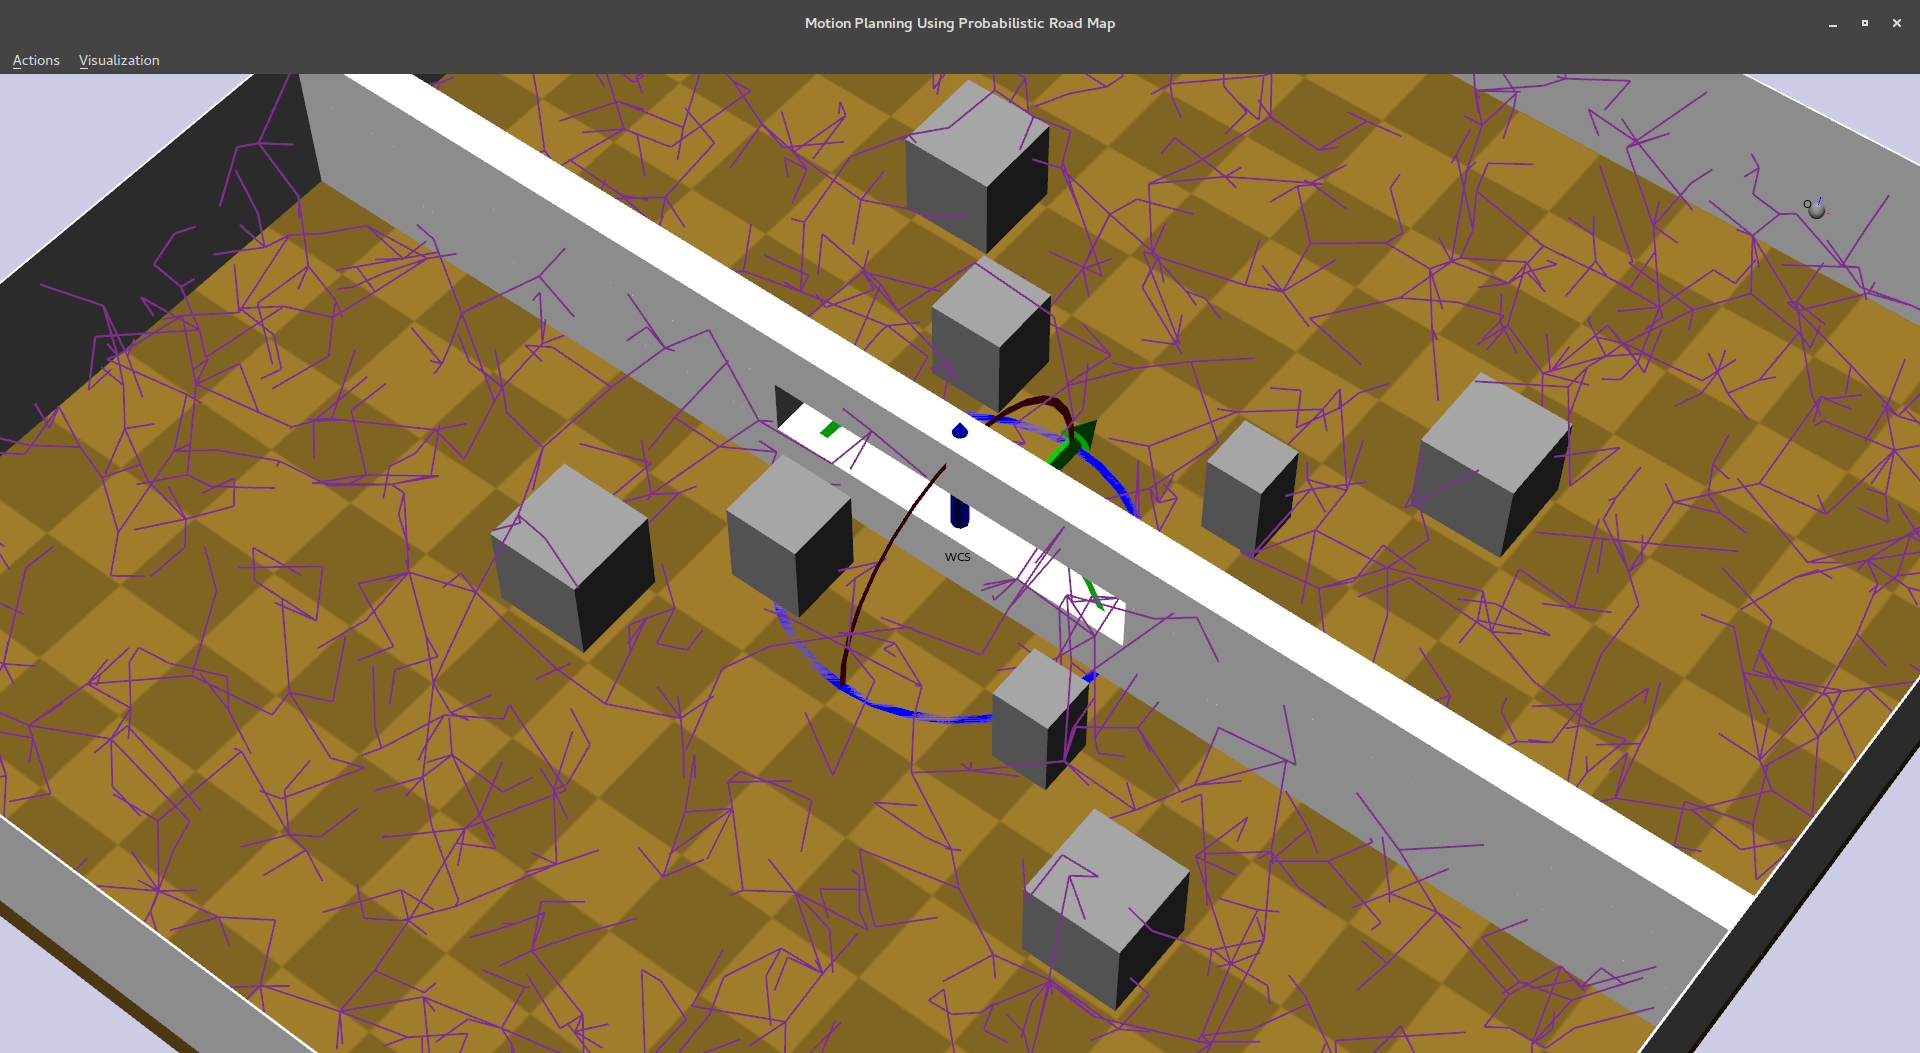
\includegraphics[width=0.8\textwidth]{prm_roadmap.png}
  \caption{Roadmap generated using PRM for one robot. The roadmap has 2000 nodes and 1980
  edges. There are 5 connected components with more than one node. There are 19 nodes
which remain disconnected.}
  \label{fig:roadmap}
\end{figure}
\subsubsection{The Expansion Step}
In the expansion step, the connectivity of the graph is improved. This is done by locating
connected components which are `difficult' based on some heuristic. It can correspond to
regions of narrow passages. The size of the connected component is used as a simple
heuristic for the project. Once such components are identified, nodes at random are
selected from these components. Then a random walk is implemented. The system of robots
move in a random direction for some distance or until hit by an object. Then the direction
is changed. The random walk is run for a specified duration. A new node is added
corresponding to the random walk. The path taken by the system of robots need to be added
to as it is obtained in a non-deterministic way.

\subsection{Query Phase}
In the query phase, an initial configuration~$\mv q_i$ and a goal configuration~$\mv q_g$
are provided. The algorithm then tries to connect to the closest node in the roadmap for
each of these configurations. If the two nodes can be connected to the roadmap, shortest
path is found between the connected nodes in the roadmap. 

The path obtained can be improved upon by applying a smoothing procedure. Two techniques
are used in this project:
\subsubsection{Greedy Approach}
First it is checked if $\mv q_i$ and $\mv q_g$ can be connected directly. If such a path
exists, the function simply returns the direct path.

If the configurations cannot be directly connected, a greedy approach is employed to
connect first node to the end node, if successful the path is shortened by directly
joining these nodes. If not the next node is checked with the last node and so on. This
greatly reduces the path taken by the system of robots.

\subsubsection{Random Approach}
A random approach is augmented with the greedy approach. Two nodes in the shortest path are checked
if they can be directly connected. If a collision-free path exists, the nodes are {\em
short-circuited}. This approach has been found to be effective for several environments.

\begin{figure}[htbp]
  \centering
  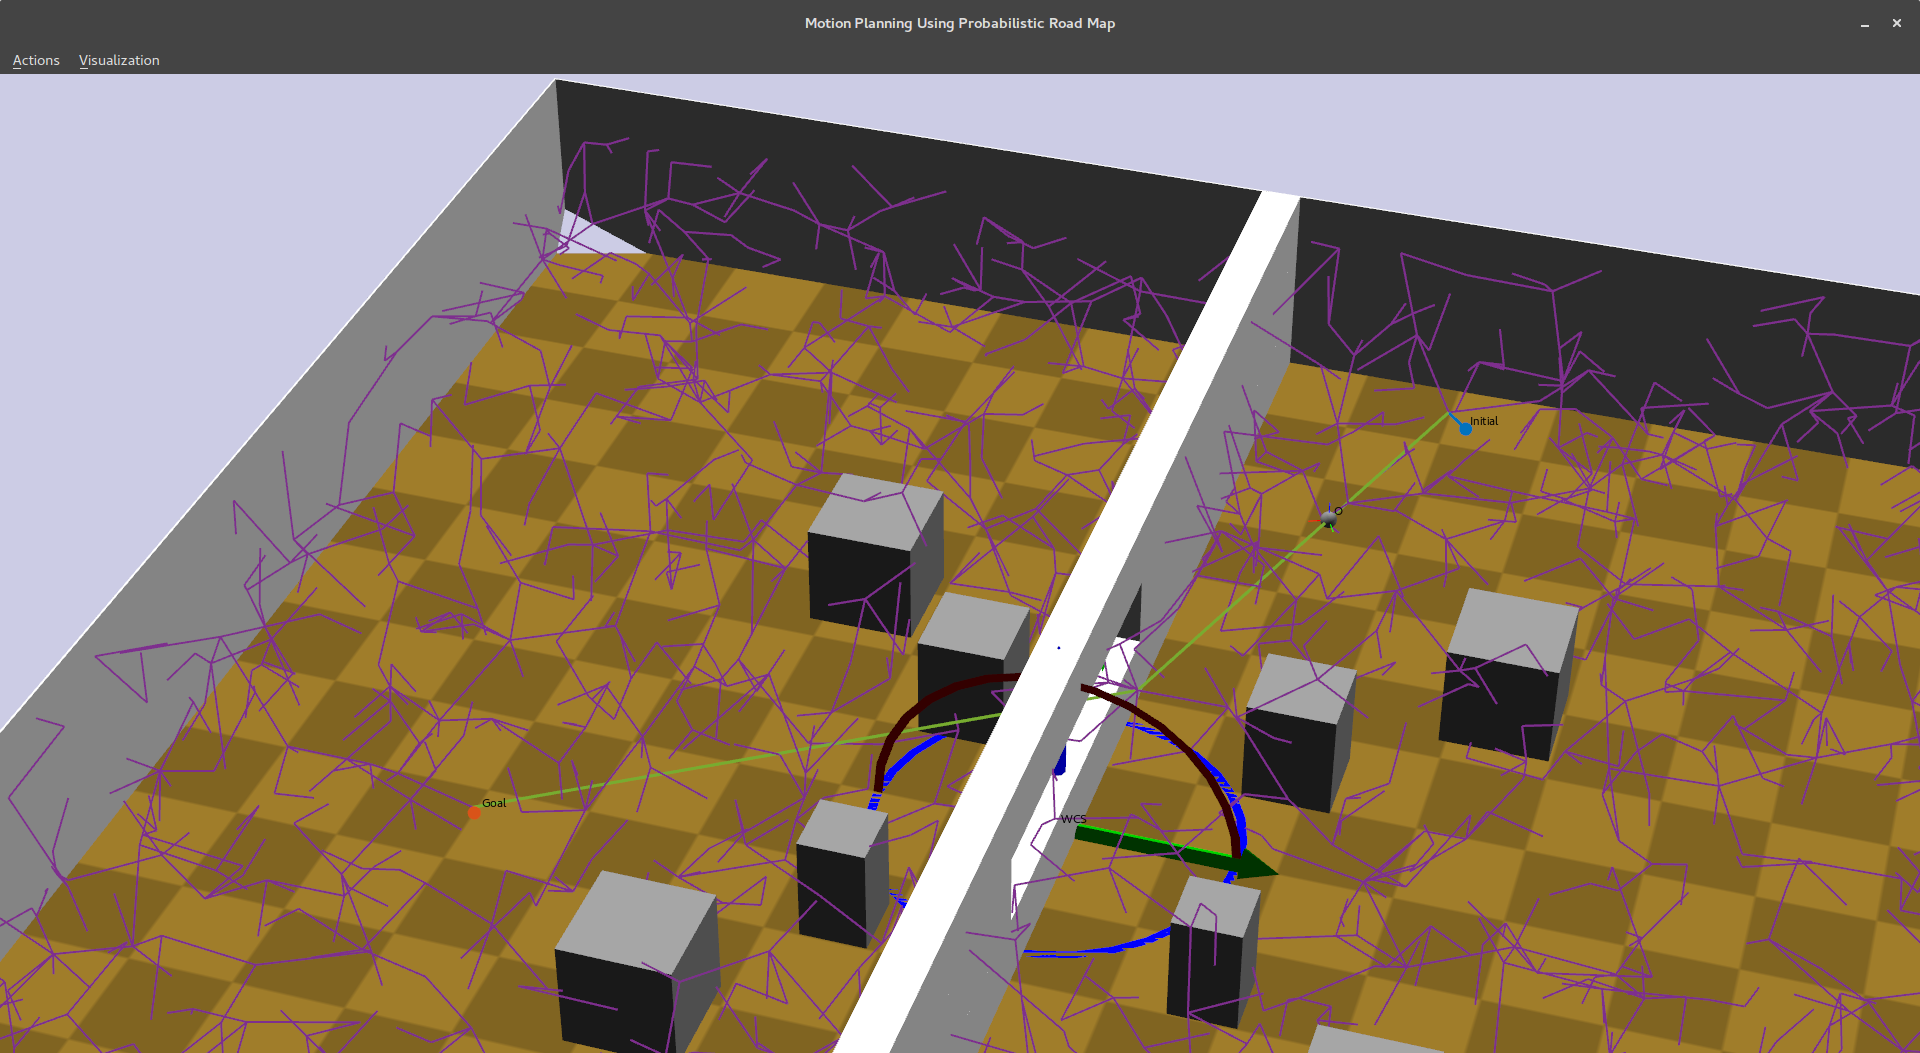
\includegraphics[width=0.8\textwidth]{path_single.png}
  \caption{A sample path for a single robot. The initial configuration is shown in blue
  and the final configuration in red. Smoothing procedure has been applied to the path to
obtain shorter paths.}
  \label{fig:pathS}
\end{figure}


\begin{figure}[bpt]
  \centerline{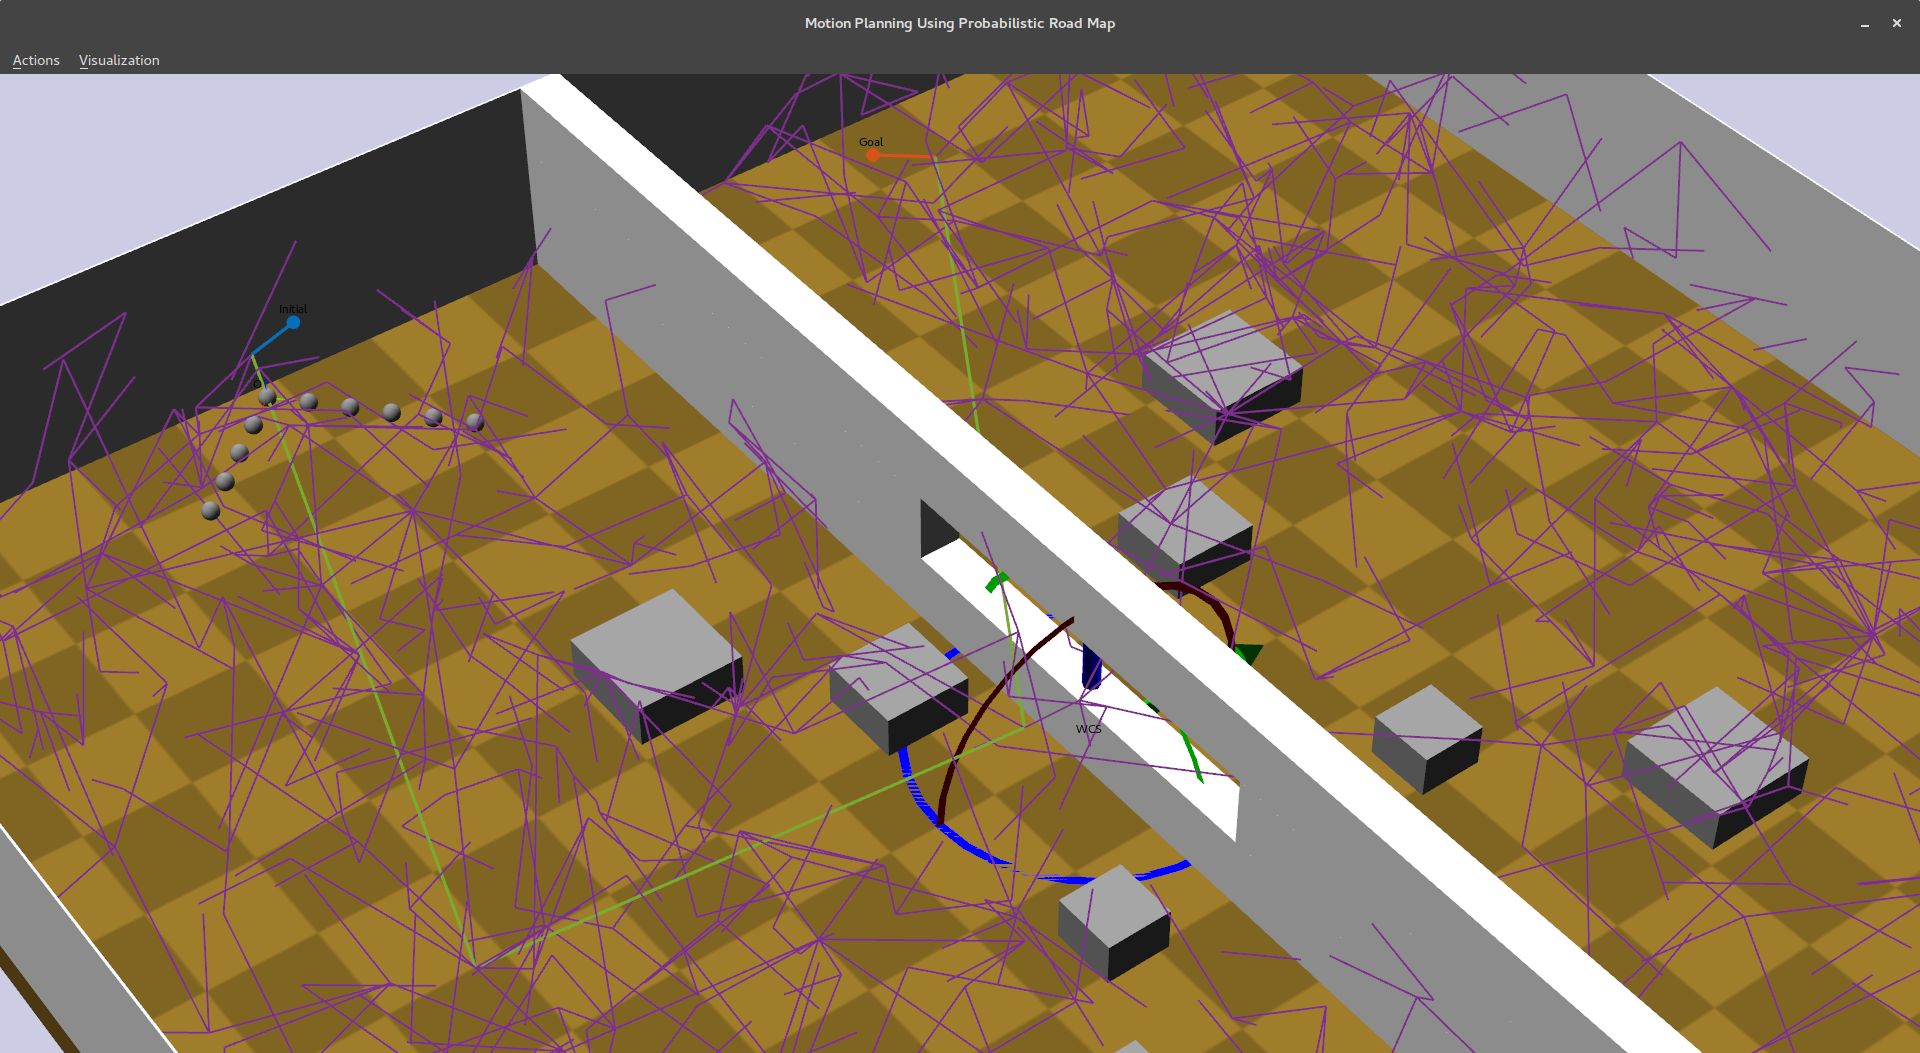
\includegraphics[width=0.45\textwidth]{lPath_start.png} %\hspace{0.01in} 
  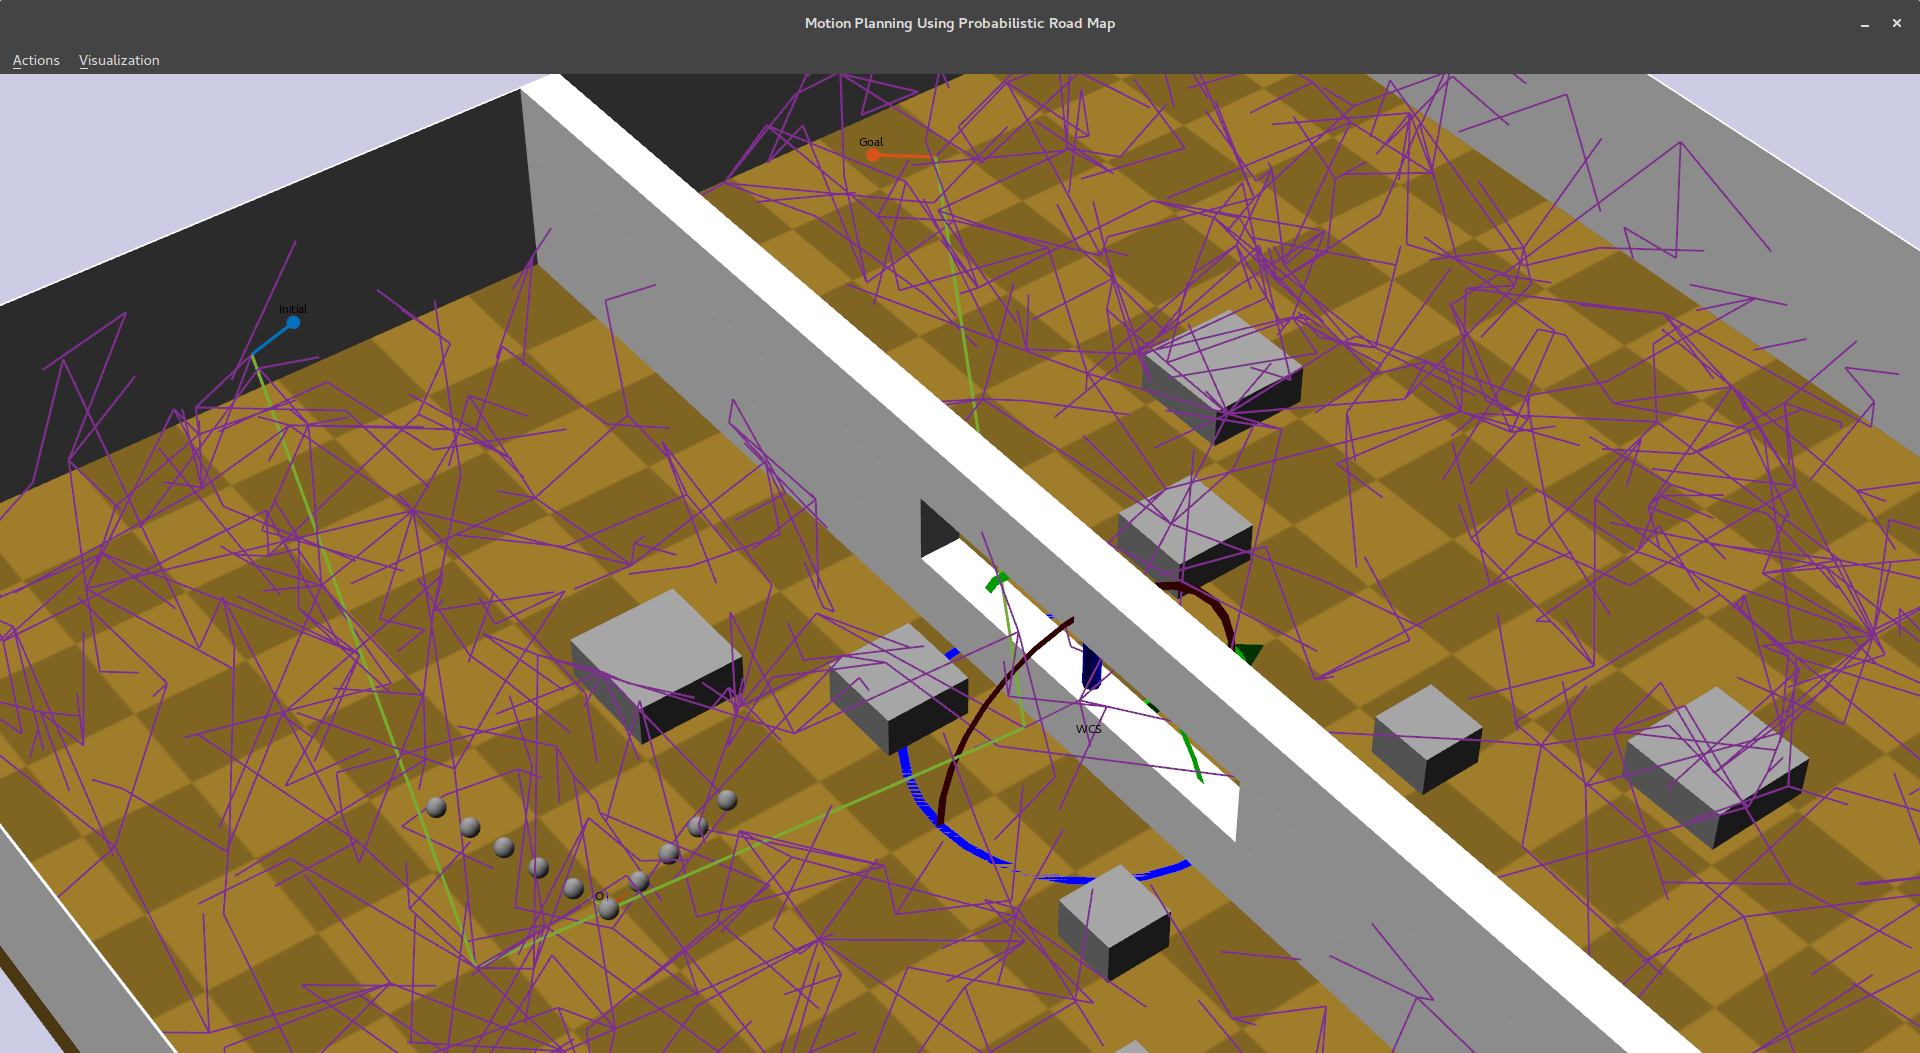
\includegraphics[width=0.45\textwidth]{lPath_mid0.png}} \vspace{0.05in}
  \centerline{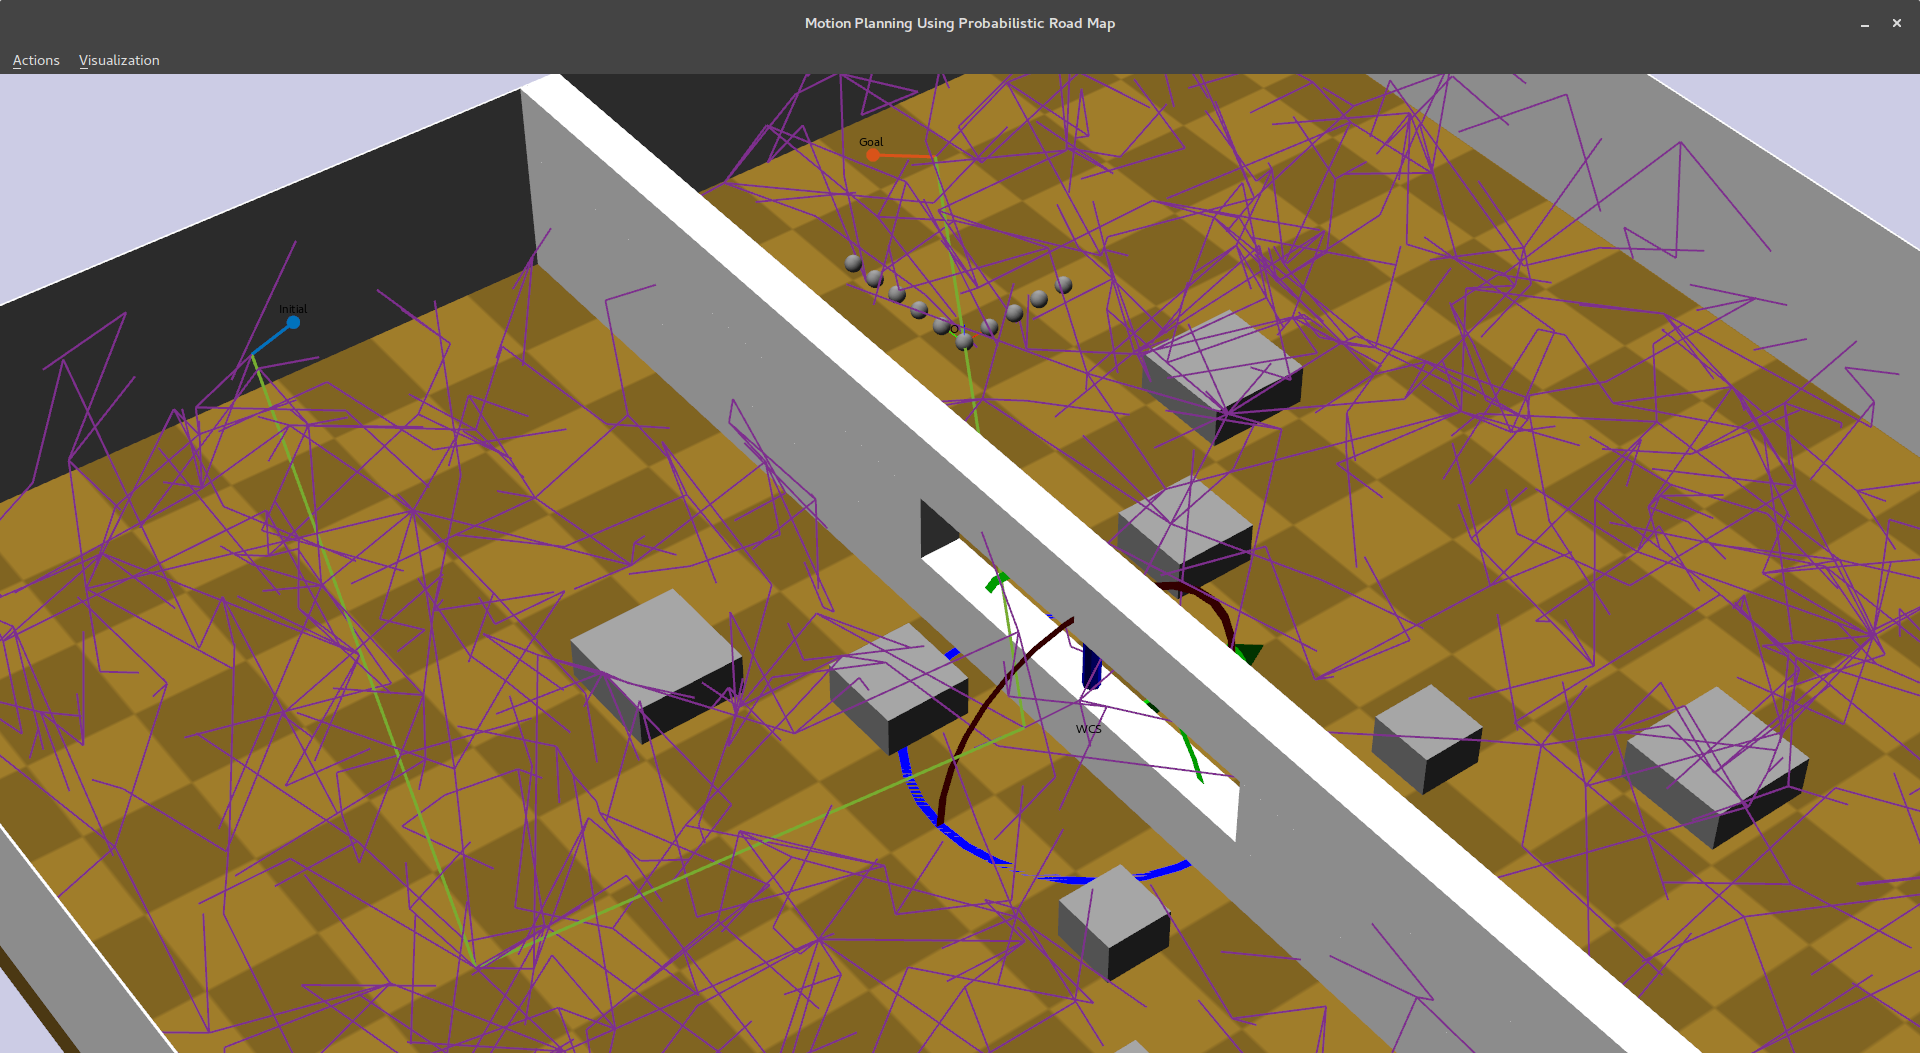
\includegraphics[width=0.45\textwidth]{lPath_mid.png} %\hspace{0.01in} 
  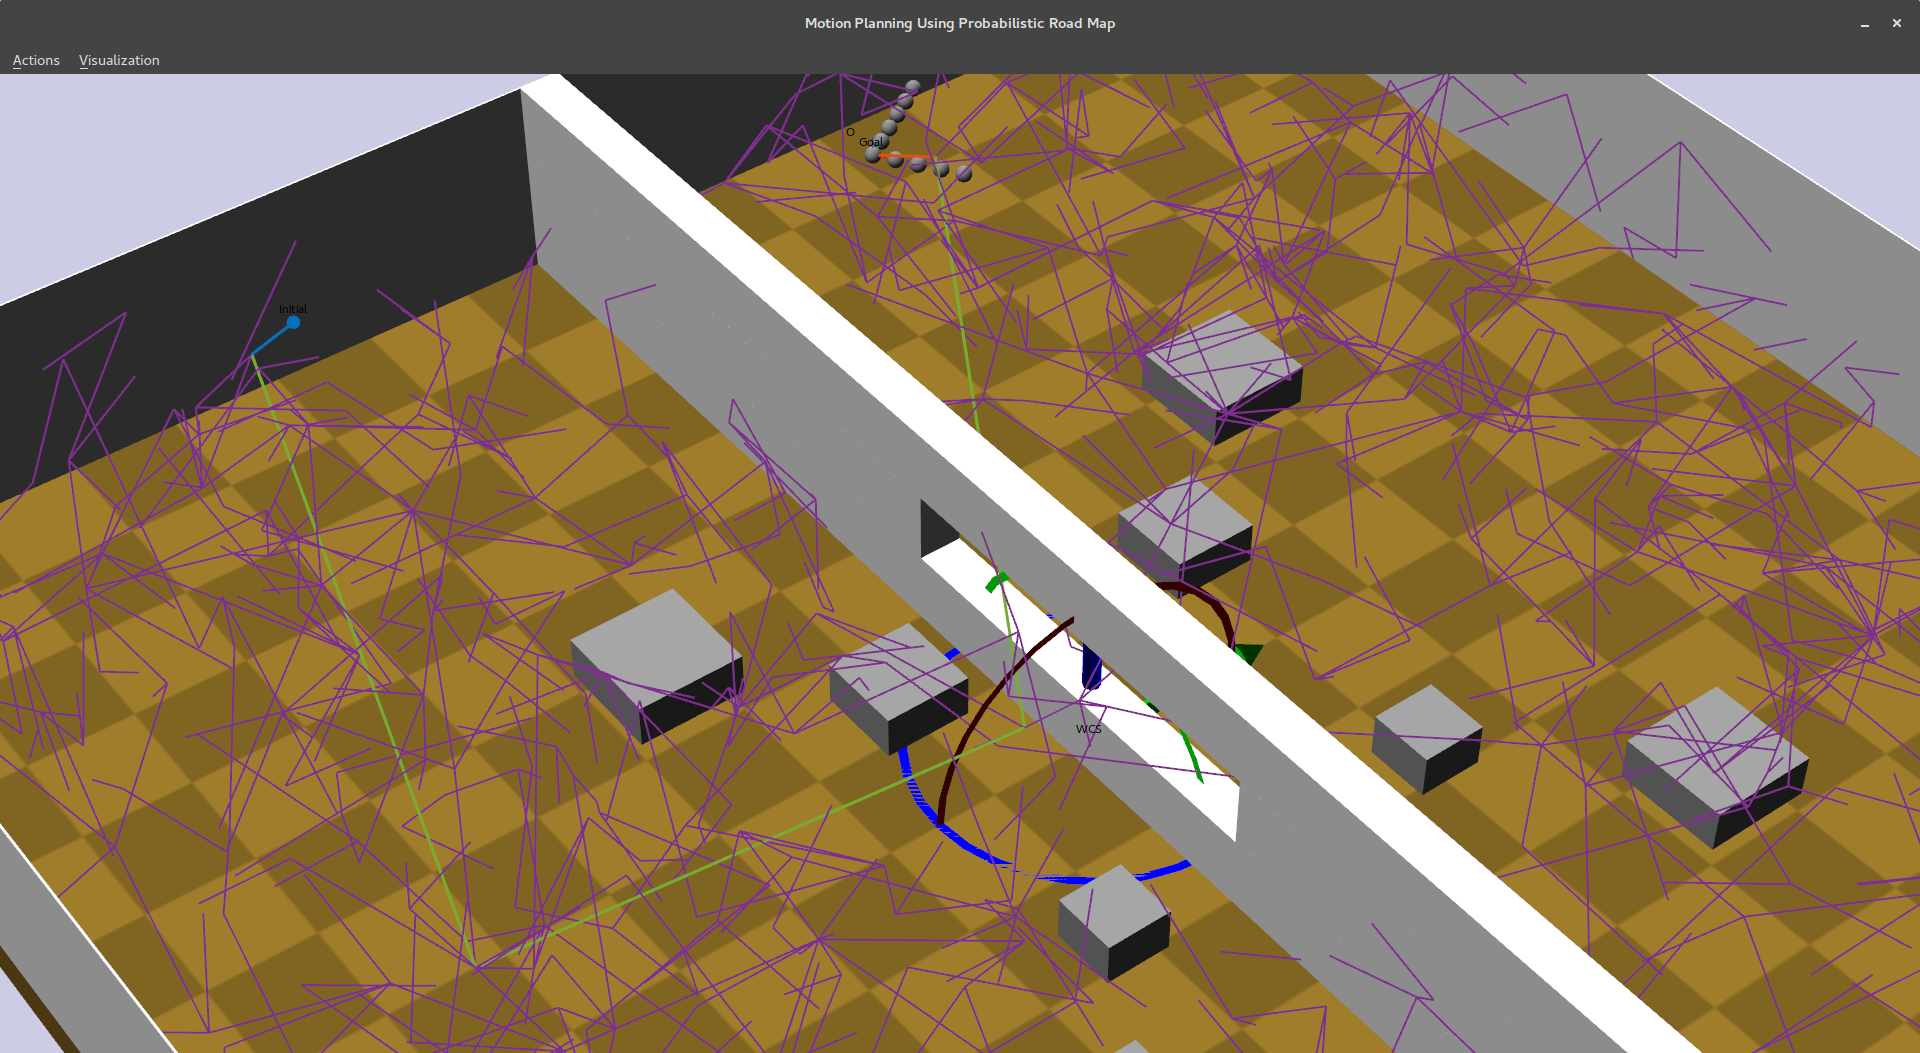
\includegraphics[width=0.45\textwidth]{lPath_end.png}}
  \caption{Path shown for 10 robots. The initial configuration is marked in blue and the
  final configuration is marked in red. The blue and and red lines show the path joining
the respective configurations to the roadmap. The final path is smoothened. Note that the
scale and orientation of the formation is also changing.}
  \label{fig:ten}
\end{figure}
\section{Experiments}
Running time experiments were performed to understand the variation in running time with
the number of robots (1--10). The environment for the experiment is shown in~\fgref{fig:env}. The
number of samples were fixed to 2000. The maximum number of nodes to connect  from a new
sample was set to 15. The neighbor hood distance was 0.75 times the number of robots. The
sampling for collision detection was set to a distance of 0.04. The query time was
averaged over 100 random queries. There were at the most 1 failure. It can be seen from
the plots that the running time in learning phase increases with increase in the number of robots. However,
the increase is not very steep. The number of nodes not connected to any other node also
increases with number of robots. This is because the size of the formation increases and
it becomes more difficult to connect configurations using collision-free path.

One interesting plot is of running time of query phase. The running time first increases
with the number of robots and then decreases. The running time is more for
3--6 number of robots. This is because of the neighborhood distance is small 
which causes the shortest path composed of several very small
segments. The complexity of the smoothing process is proportional to the number of
segments in the shortest path. Hence, the running time increases for smaller number of
robots. The running time increases for 1--4 robots because the collision detection is
implemented to ensure the paths are collision free.

\begin{figure}[htbp]
  \centering
  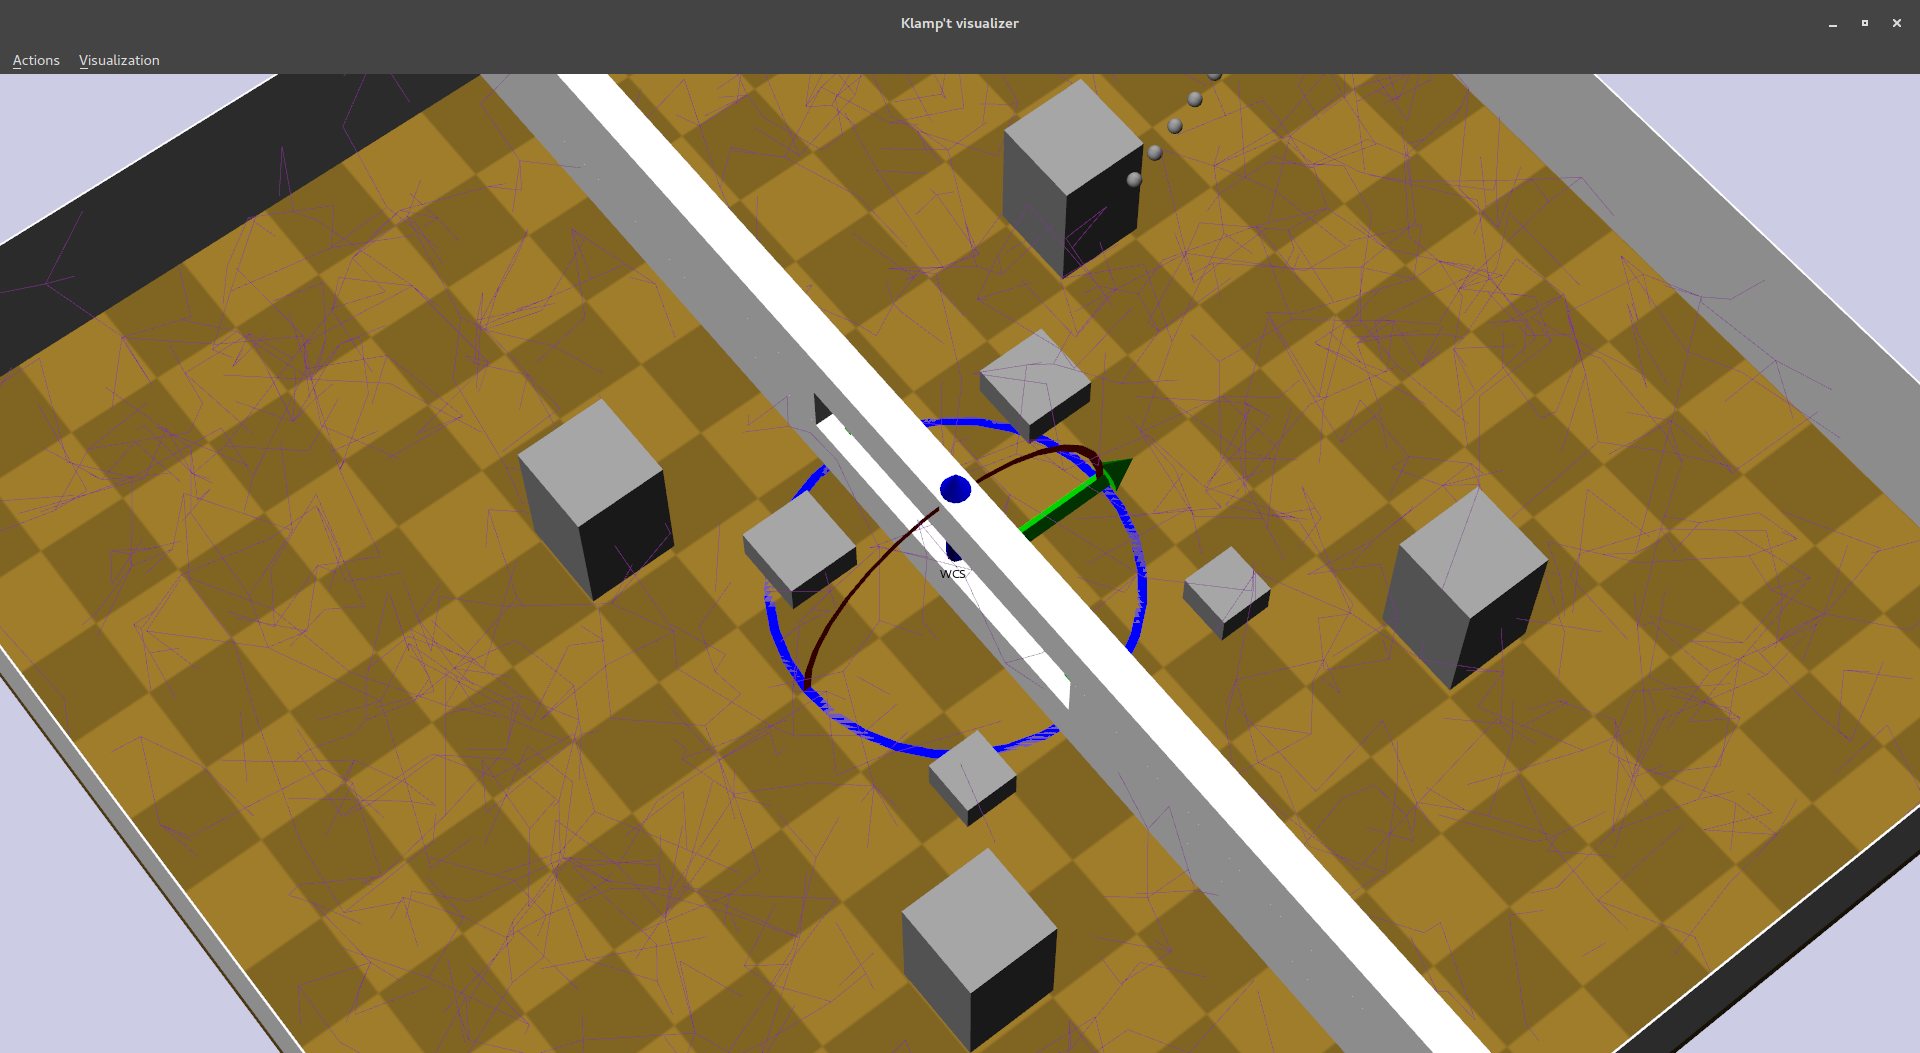
\includegraphics[width=0.8\textwidth]{env.png}
  \caption{Environment setup for the experiments}
  \label{fig:env}
\end{figure}
\begin{figure}[htbp]
  \centering
  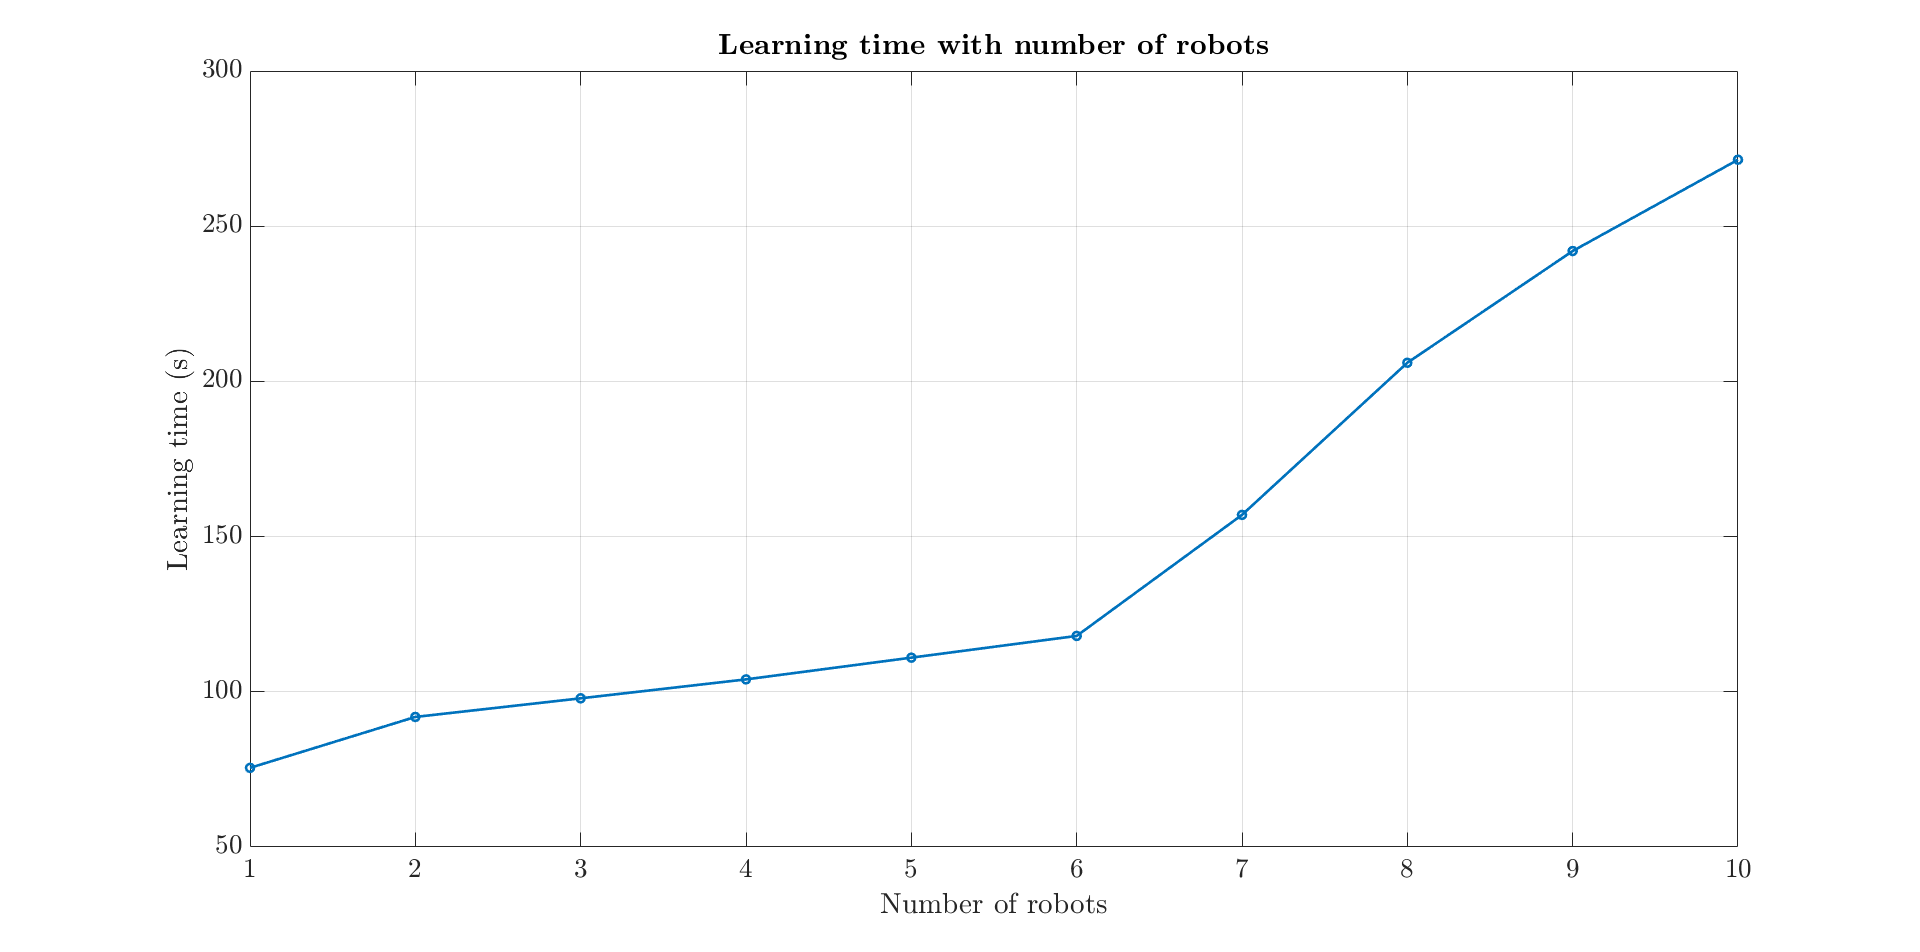
\includegraphics[width=0.8\textwidth, trim={4cm 0 4cm 0},clip]{lT_plot.png}
  \caption{Variation of running time of learning phase with number of robots. }
  \label{fig:lT}
\end{figure}

\begin{figure}[htbp]
  \centering
  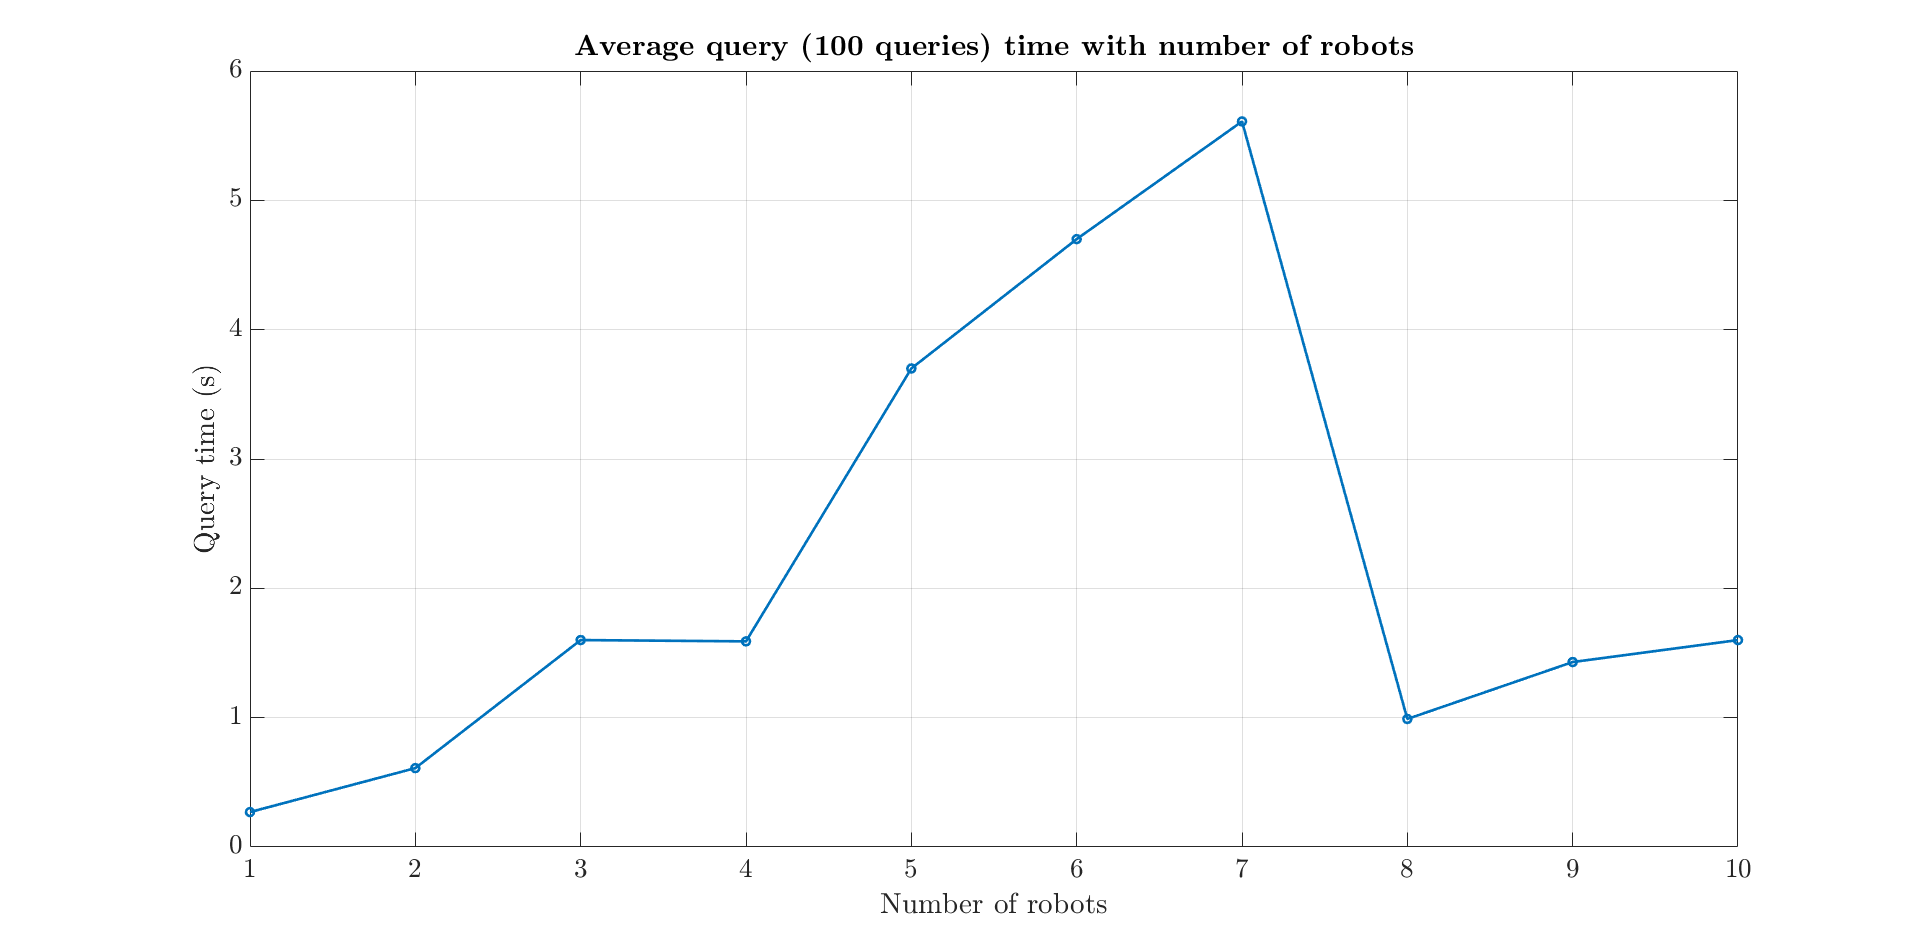
\includegraphics[width=0.8\textwidth, trim={4cm 0 4cm 0},clip]{qT_plot.png}
  \caption{Variation of running time of query phase with number of robots. }
  \label{fig:qT}
\end{figure}

\begin{figure}[htbp]
  \centering
  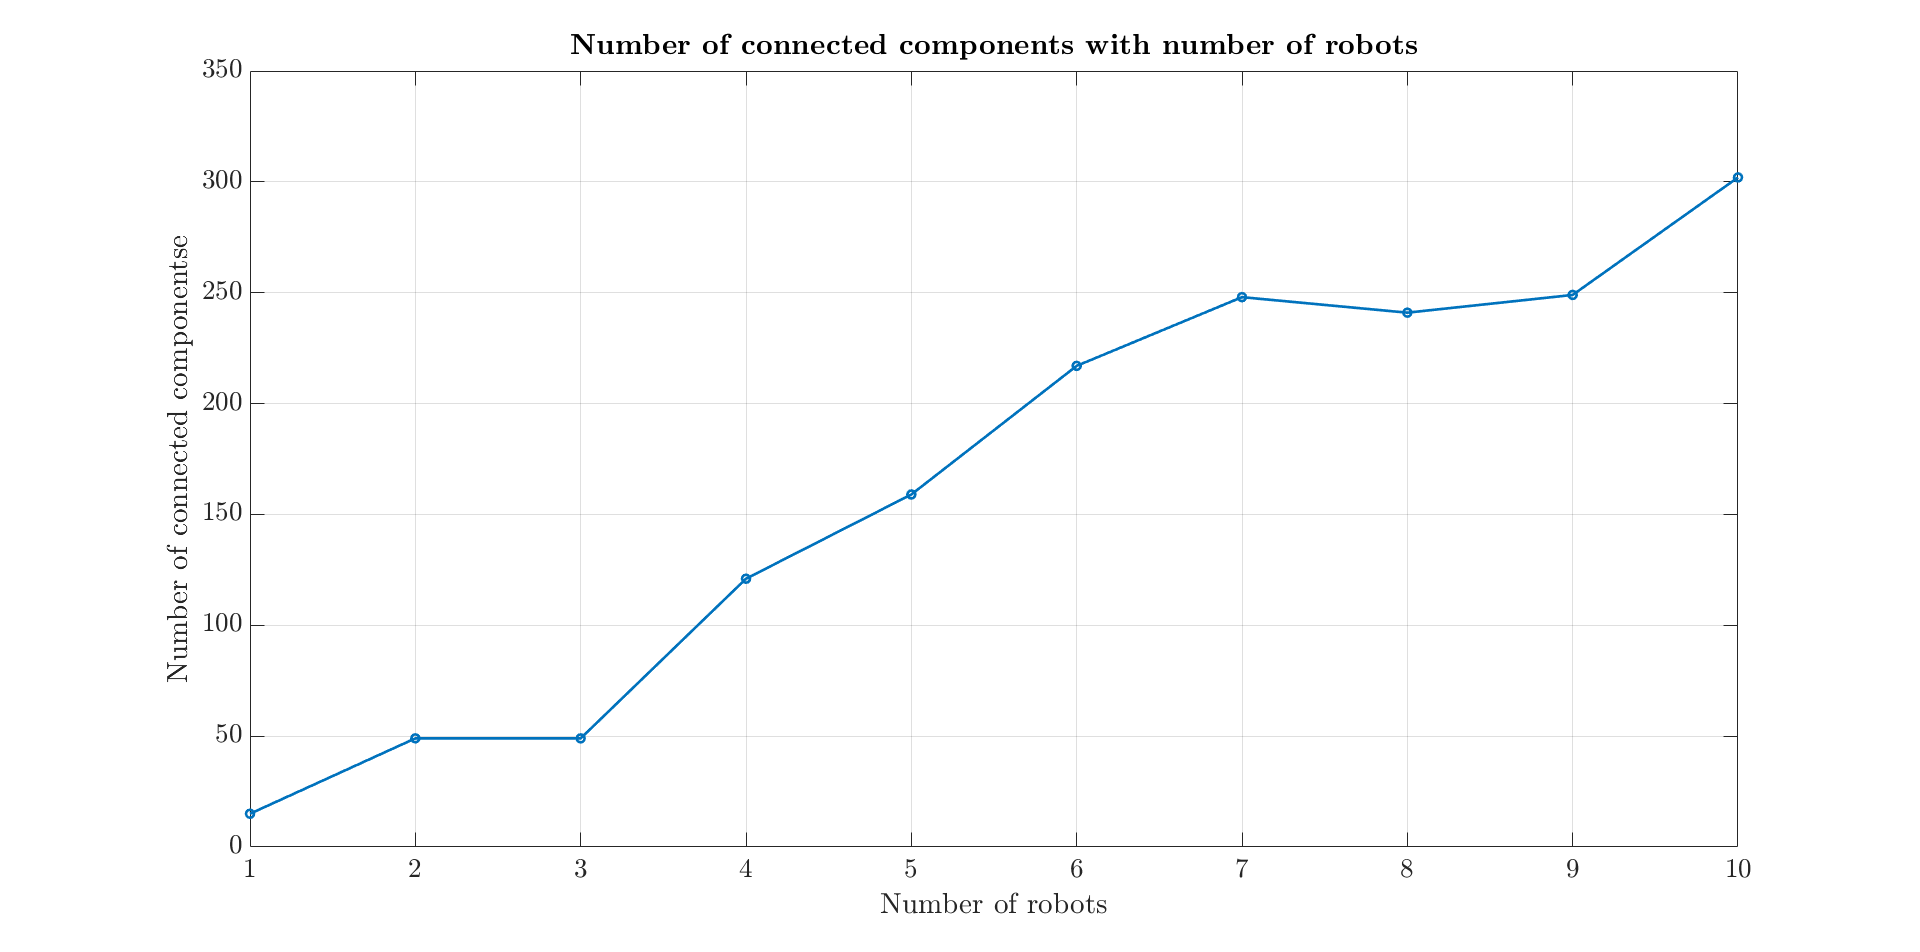
\includegraphics[width=0.8\textwidth, trim={4cm 0 4cm 0},clip]{cc_plot.png}
  \caption{Variation of number of connected components with number of robots. }
  \label{fig:cc}
\end{figure}

\begin{figure}[htbp]
  \centering
  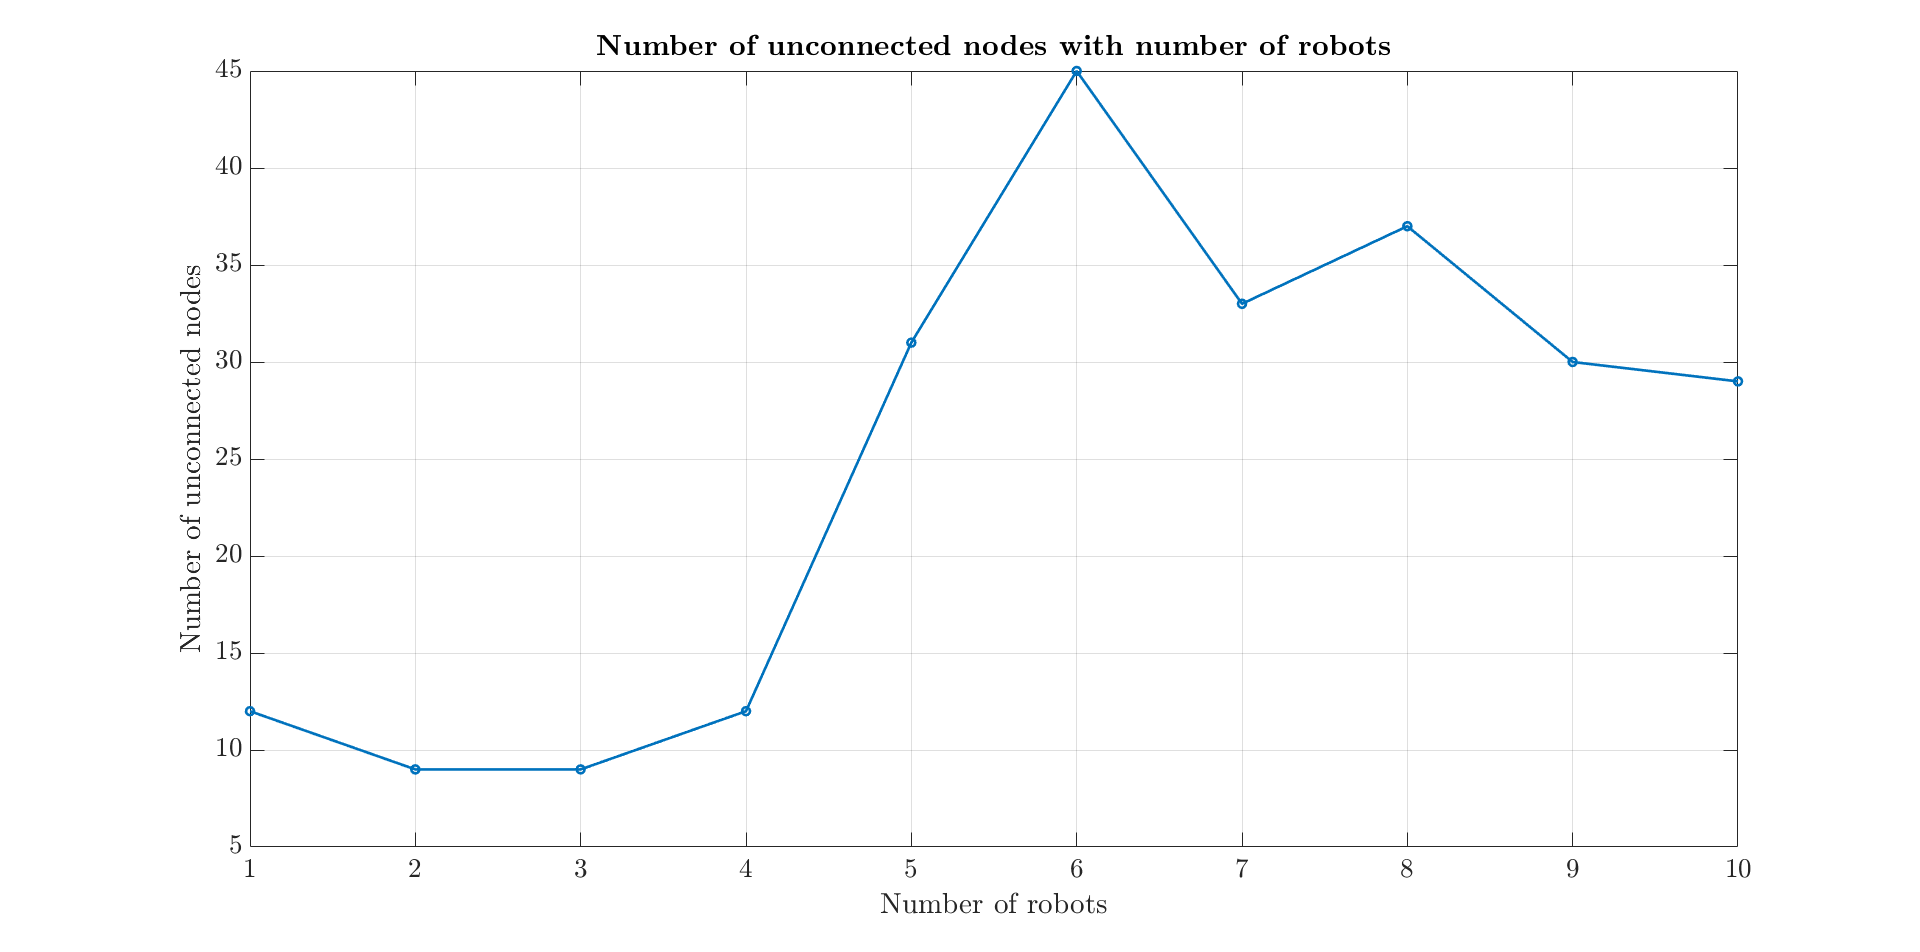
\includegraphics[width=0.8\textwidth, trim={4cm 0 4cm 0},clip]{ccn_plot.png}
  \caption{Variation of number of unconnected nodes with number of robots. }
  \label{fig:ccn}
\end{figure}

\bibliographystyle{IEEEtran}
\bibliography{bibNmacro/agarwal_MP}

\end{document}
